
% Research question here?
% Going to be challenging to have this not come across as a software design
% spec.. Let's try to get this section over with as little text wasted as
% possible... I feel silly writing these sections, since I ALWAYS skip over
% them when I'm reading other people's papers...
\projectname{} is our realization of correspondence checking and \simulator{}
as a useful platform to troubleshoot SDN controllers. In this section we discuss
our goals in designing \simulator{}, and the challenges we encountered in the process
of realizing these goals.

\subsection{Design Goals: The 7 rules of \projectname{}}

We seek to build a system that facilitates the process of troubleshooting.
First and foremost, we hope that \projectname{} can reproduce difficult bugs
observed in production networks, and automate the process of diagnosing their
causes. We also envision \projectname{} being used as a common repository for difficult, corner-case
scenarios known to have caused problems for other control platforms in the past.
Given these potential use cases, we require the design of the system to be
driven by the following requirements:

\noindent{\bf (1) Realistic Network Sizes.} We focus on large, production SDN
deployments. As today's datacenters may contain up to 100,000 hosts and 10,000
switches, our simulation infrastructure must be able to support large numbers
of switches.

\noindent \textbf{(2) Control plane focus} We expect the dynamism in our system to stem from
\emph{control plane events}. Typical rates of control plane events must thus be
handled, and control plane events must be modeled precisely. Conversely, we
don't expect to handle a realistic amount of dataplane traffic, which is
intractable for a software solution, and largely irrelevant in current networks (because they are mostly proactive, so control planes are not being driven by packet arrivals).

\noindent \textbf{(3) Controller choice} Our system should run with existing production
controllers with minimum additional instrumentation. To allow for wider adoption, we don't want to limit ourselves to
a particular controller implementation.

\noindent \textbf{(4) Full determinism} We want our simulation environment to be fully
deterministic, such that repeated simulations with identical initialization values
yield provably identical results. This creates a challenge in conjunction with our goal (3).

\noindent{\bf (5) Comprehensive Failure Modes.} \projectname{} should
support a wide range of failure modes at all components in the
system, including switch and link failures and message drops, delays and reorderings.

\noindent\textbf{(6) Corner cases investigation} The potential state-space in a large-scale network
is intractably large \colin{Reviewer OD: do a better job of describing the
relationship of our work to model checking}.  We focus on interesting cases, as recorded, e.g., in production, or
found through interactive evaluation. To investigate related error conditions,
we \emph{fuzz} the input traces.

\noindent\textbf{(7) Interactivity} The system should be fast enough for interactive exploration through
an operator.

\medskip

While none of these requirements were particularly difficult in isolation, taken in aggregate they posed some difficulties, as we now recount.

\subsection{Components}

As depicted in Figure \ref{fig:system}, \projectname{} combines several
components to facilitate the process of troubleshooting SDN platforms:
\projectname{} takes input
from production traces, interactive manipulation, and synthetic trace
generation, and fuzzes these inputs to ensure that fixes are sufficiently general;
\projectname{}'s simulator supports large, sophisticated networks;
\projectname{} provides a deterministic, code-agnostic execution environment
for running SDN control software; and provides efficient algorithms for
checking correspondence throughout the system execution. We now provide an
overview of each of these components, and the challenges we encountered in
realizing our goals.

\begin{figure*}[!t]
  \centering
  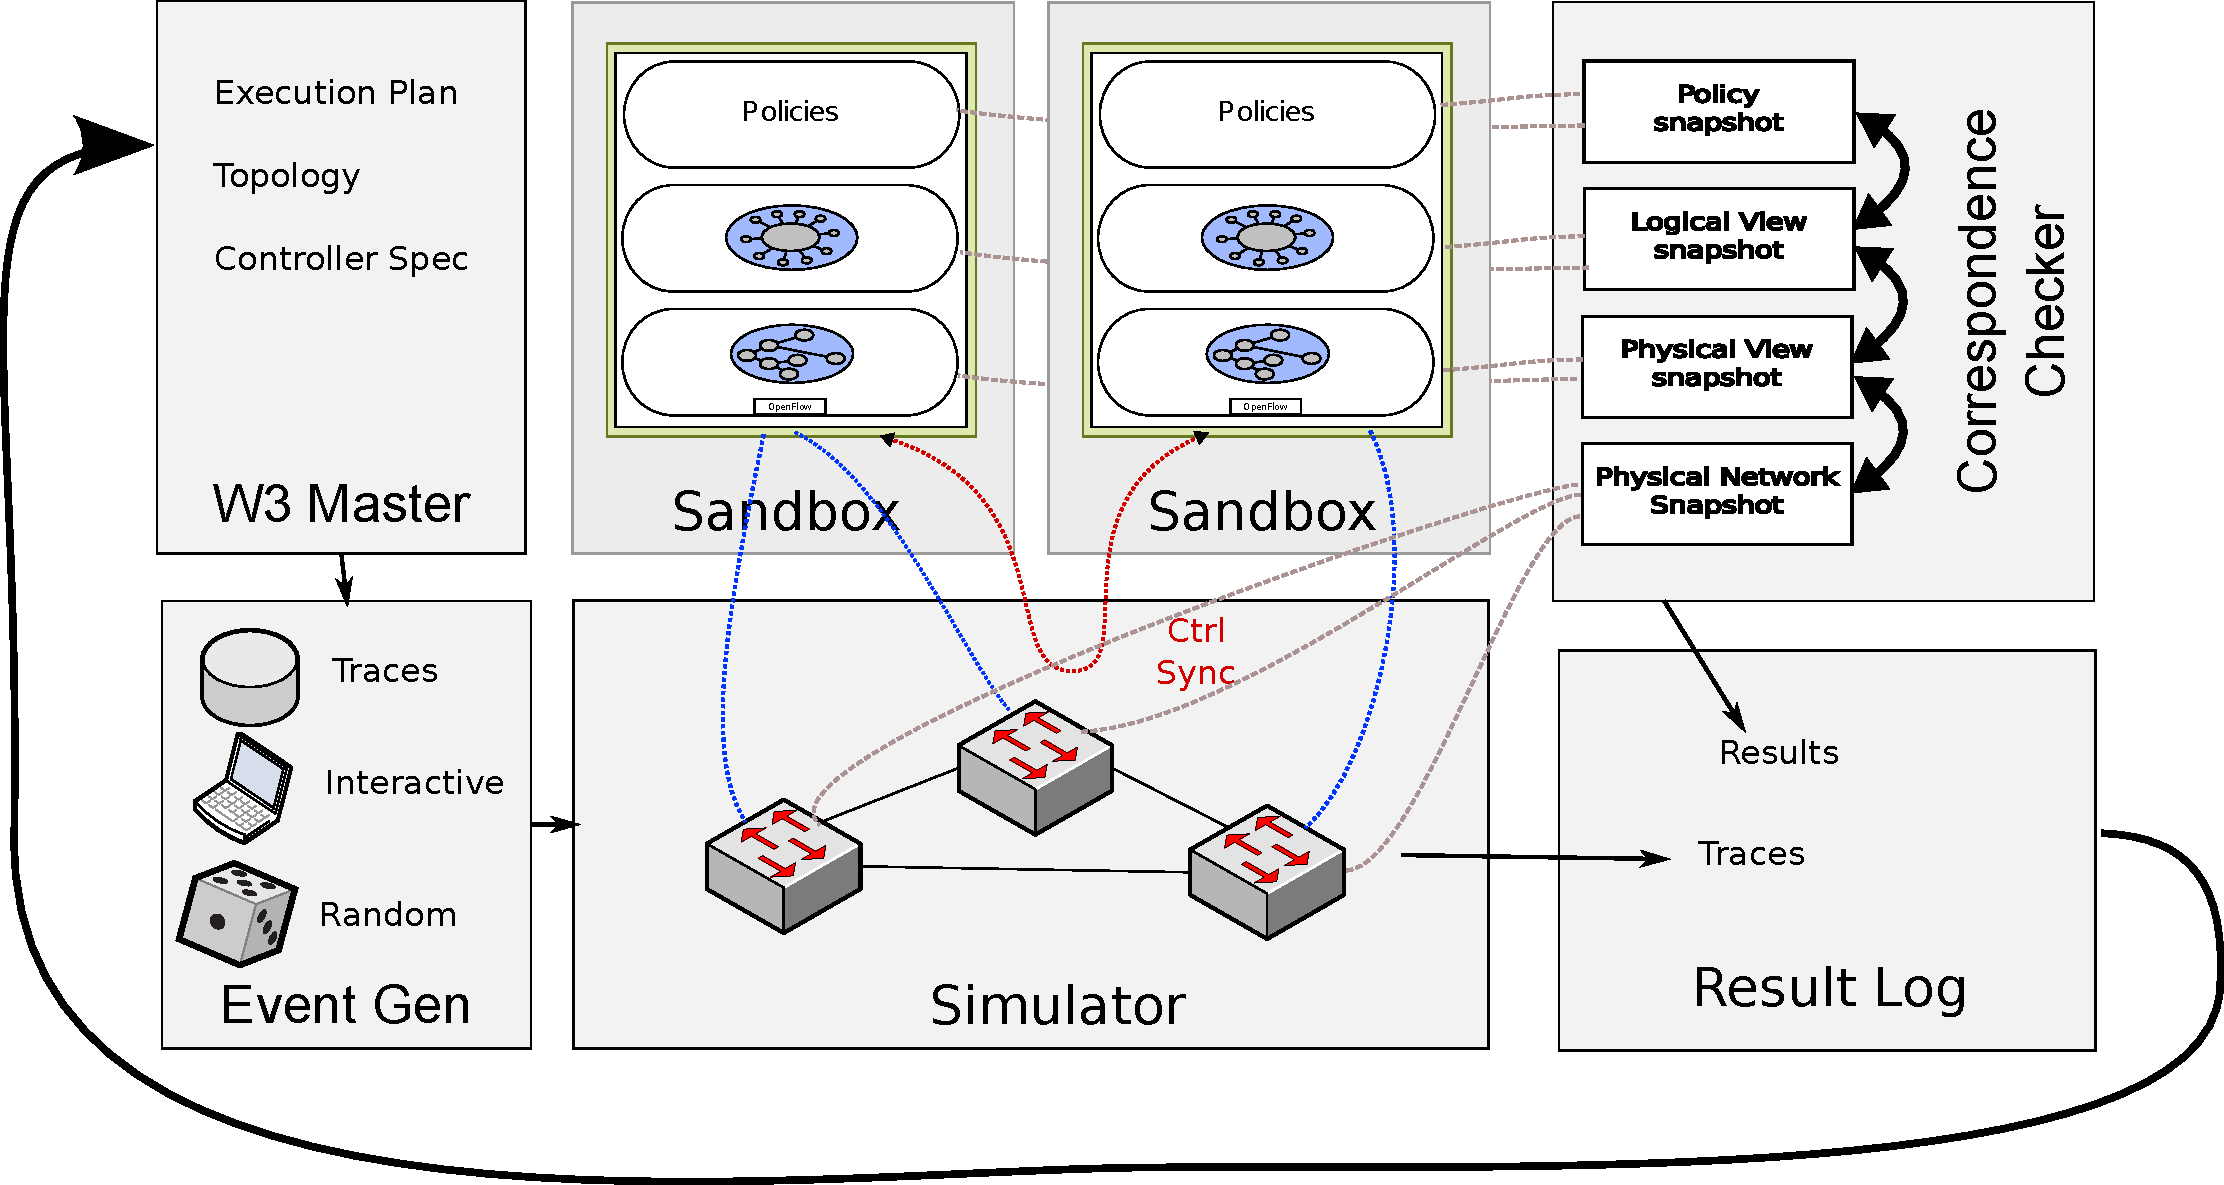
\includegraphics[width=0.8\textwidth{}]{../diagrams/architecture/architecture.pdf}
  \caption{System architecture. \colin{Andi: can haz new diagram? :P}}
  \label{fig:system}
\end{figure*}

\noindent{\bf Trace Input And Fuzzing.} Since a major goal of \projectname{} was
to support a wide range of usage scenarios, % WAT does that even mean
we provide support for three different methods for generating network trace
inputs. The most common method is to insert failure and topology change logs
from production deployments into the simulator for replay. Input traces may
also be produced synthetically with configurable, random probabilities for
network events. Lastly, we support interactive use, where the troubleshooter
has complete control over network events, and is thereby free to explore her
intuitions in order to reproduce a failure mode she has in mind.

\noindent{\bf Simulator.} We have built a simulator for SDN networks,
where network devices and hosts are modeled as lightweight python objects.
\colin{Reviewer OA: python objects creep in to the writing} Within a single thread, we
are able to deterministically model the execution of very large networks.
Our simulated model supports a wide
range of failure modes, and provides fine-grained control over event
orderings, component failures, and other aspects of the system execution. Our
simulator currently supports switch failures, link failures, arbitrary packet
re-orderings, drops and delays, and a fully general control plane.

The main challenge we encountered in the design of the simulator was
maintaining large numbers of TCP connections to the
controller(s). Although the controllers themselves may be spread
over multiple physical servers, the main simulator must nonetheless handle all
TCP connections between switches and controllers within a single process.
We ultimately ended up using epoll to avoid limitations of the UNIX select
implementation.

\noindent{\bf Controller Sandbox.} One of our major goals for \projectname{}
was to be able to run any SDN controller on top of the platform, with minimal
code changes to the controllers themselves. In addition, control servers
running on top of the simulated network must support deterministic execution
for reproducible results.

Currently we run applications as UNIX processes outside of the simulator.
We note however that there are a number of approaches for achieving deterministic
replay for external software. For example: a software determinism layer (e.g.
deterministic random number generators \colin{Reviewer OA: Whenever I see
replay, I worry about dealing with nondeterminism and pseudorandom number
generators. It was not clear how you are dealing with these issues.}) is
extremely lightweight, but requires modifications to the external software;
binary rewriting does not require any modification to the external
software's source code, but incurs moderate performance overhead; and VMs
fully support deterministic replay, but only a relatively small number of VMs can be run
on a single machine. We hope to leverage this previous work in future versions
of \projectname{}. Nonetheless, our architecture does not prevent us from
running controllers on different physical
servers in case we encounter memory or CPU bottlenecks.

\noindent{\bf Correspondence Checking.}
\projectname{} leverages the Hassel library provided by HSA~\cite{hsa}
to implement the correspondence checking algorithm. We optimize the code
slightly to run efficiently on large networks; in particular, we parallelize
symbolic packet propagation to a large number of subtasks. Correspondence
checking currently requires a small code change to the controller to fetch
the platform's view of the network state.

\projectname{} is written in roughly 5,000 lines of python, and is publicly
available. [anon]
